\documentclass[12pt,a4paper,titlepage,oneside]{report}
\usepackage[T1]{fontenc}
\usepackage{titlesec, blindtext, color}
\usepackage[spanish]{babel}
\usepackage[utf8]{inputenc}
\usepackage{lmodern}
\usepackage{graphicx}
\usepackage{subcaption}
\usepackage{pdfpages}
\usepackage{xcolor}
\usepackage{color}
\usepackage{url}
\usepackage{pdfpages}
\usepackage{fourier} % Use the Adobe Utopia font for the document - comment this line to return to the LaTeX default
\usepackage{amsmath,amsfonts,amsthm} % Math packages
\usepackage{listings}
\usepackage{caption}
\usepackage{titling}
\usepackage{lipsum} 
\usepackage{sectsty}
\usepackage{fancyhdr}
\usepackage{float}
\usepackage{tabulary}
\usepackage[colorlinks=true,linkcolor=black,urlcolor=blue,citecolor=black]{hyperref} 
\usepackage{booktabs}% http://ctan.org/pkg/booktabs
\usepackage{pgfplots}

\pagestyle{fancy}
\fancyhf{}
%\fancyhead[LE,RO]{\nouppercase \leftmark}
\fancyhead[LO,RE]{\nouppercase \rightmark}
\fancyfoot[C]{\thepage}

\newcommand{\Keywords}[2]{\vfill\noindent{\small{\em Palabras clave}: }}
\newcommand{\KeywordsEn}[2]{\vfill\noindent{\small{\em KeyWords}: }}
\definecolor{grisclar}{gray}{0.5}
\definecolor{grisfosc}{gray}{0.25}

% Editar con los datos correspondientes
\newcommand{\titulo}{Sistema Autónomo de Riego y Monitorización de un Cultivo}
\newcommand{\titulacion}{Máster de Ingeniería Informática}
\newcommand{\autor}{Carlos Barranco , Alexander Quesada López}
%\newcommand{\director}{}

% Colors definitions

\definecolor{mygray}{rgb}{0.9,0.9,0.9} % Color definition
\definecolor{darkspringgreen}{rgb}{0.09, 0.45, 0.27}
\definecolor{babyblue}{rgb}{0.54, 0.81, 0.94}
\definecolor{airforceblue}{rgb}{0.36, 0.54, 0.66}
\definecolor{blue(ncs)}{rgb}{0.0, 0.53, 0.74}
\definecolor{gray75}{gray}{0.75}

\title{\titulo}
\author{\autor}
\renewcommand\chaptername{IOT}

\newcommand{\hsp}{\hspace{15pt}}
\titleformat{\chapter}[hang]{\Huge\bfseries}{\thechapter\hsp\textcolor{gray75}{|}\hsp}{0pt}{\Huge\bfseries}


%Comment -> Ctrl+T
%Uncomment -> Ctrl+U

\begin{document}
\begin{titlepage}
\begin{center}

\begin{minipage}{0.49\linewidth}
\begin{flushleft}

\includegraphics[height=1.5cm]{./images/logo_uhu}
\end{flushleft}
\end{minipage}
\begin{minipage}{0.49\linewidth}
\begin{flushright}

\includegraphics[height=1.5cm]{./images/logo_etsi}
\end{flushright}
\end{minipage}

\vspace{2cm}

\begin{color}{grisfosc}
\large
Escuela Técnica Superior de Ingeniería\\[0.2cm]
Universidad de Málaga\\[1.9cm]
\end{color}

% Título del proyecto y titulación
{\LARGE \bfseries \titulo}\\[1.5cm]
\textsc{\large Trabajo de prácticas}\\[0.4cm]
\textcolor{grisclar}{\large\titulacion}\\[5.0cm]

% Autor, director y fecha
\begin{flushright} \large
\emph{Autor:} \autor\\[0.4cm]
%\emph{Director:} \director\\[0.6cm]
\today
\end{flushright}

%\vfill
% Bottom of the page
%{\large \today}

\end{center}

\end{titlepage}


\lstset{ 
	  backgroundcolor=\color{white},
	  basicstyle=\footnotesize, 
	  breakatwhitespace=false, 
	  breaklines=true,     
	  captionpos=c,    
	  commentstyle=\color{darkspringgreen},
	  extendedchars=true,  
	  keepspaces=true,
	  keywordstyle=\color{blue},       % keyword style               
	  numbers=left,            
	  numbersep=7pt,  
	  rulecolor=\color{black},
	  showspaces=false,
	  showstringspaces=false,
	  showtabs=false,
	  stringstyle=\color{blue(ncs)},     % string literal style
	  tabsize=2	
}

\tableofcontents
\listoffigures

\chapter{Contexto y Descripción}
	El objetivo de este proyecto es desarrollar un prototipo basado en tecnologías de IoT (Internet of Things) para el control de un cultivo equipado con un sistema de riego inteligente. Por tanto, el usuario podrá conocer en todo momento las condiciones ambientales en las que se encuentra el cultivo y consultar el histórico de las mediciones realizadas. Además el sistema garantizará que el cultivo poseerá el agua necesaria en todo momento de forma inteligente y eficiente, ya que se tendra en cuenta tanto las condiciones actuales como las previsiones meteorológicas. Para ello, a modo de prototipo se diseñará y construirá una jardinera adaptada capaz de soportar un cultivo y a la que sea posible adaptar los elementos IoT necesarios.


	Este dispositivo de encargará de medir los parámetros básicos para las plantas (temperatura, humedad aire, humedad suelo,...) a través de sensores, y en función del tipo de cultivo y los valores registrados  se activará el sistema de riego del sistema. En una segunda fase, se podrán incluir otras funcionalidades como el aviso al usuario cuando en algunos de los parámetros registrados se sobrepasen valores umbrales vía mail.



\chapter{Esquema básico del hardware}

	El núcleo del sistema hardware estará compuesto por un dispositivo una Raspberry Pi y el ESP8266 al que se interconectarán los sensores y actuadores necesarios para el sistema. Por tanto, el dispositivo ESP8266 se encargará de la lectura de los diferentes sensores junto a la actuación y decisión de activar los actuadores correspondientes. Por ejemplo, si es necesario activar el sistema de riego.

	Por otro lado, el usuario podrá interactuar con el sistema a través de un cuadro de mandos desarrollado en Node-Red, que se instalará en la Raspberry, la cual a su vez estará conectada al ESP8266. \cite{ruiz}
	
	A modo de ejemplo, en la siguiente figura se muestra el esquema general de la solución donde se ha ubicado un sensor de humedad del suelo, en función de las mediciones del mismo se decidirá si es necesario activar la bomba de agua para que sea posible regar el cultivo.

Siguiendo este esquema, se conectarían al sistema el resto de sensores y actuadores necesarios.
	
	\begin{figure}
		\center
		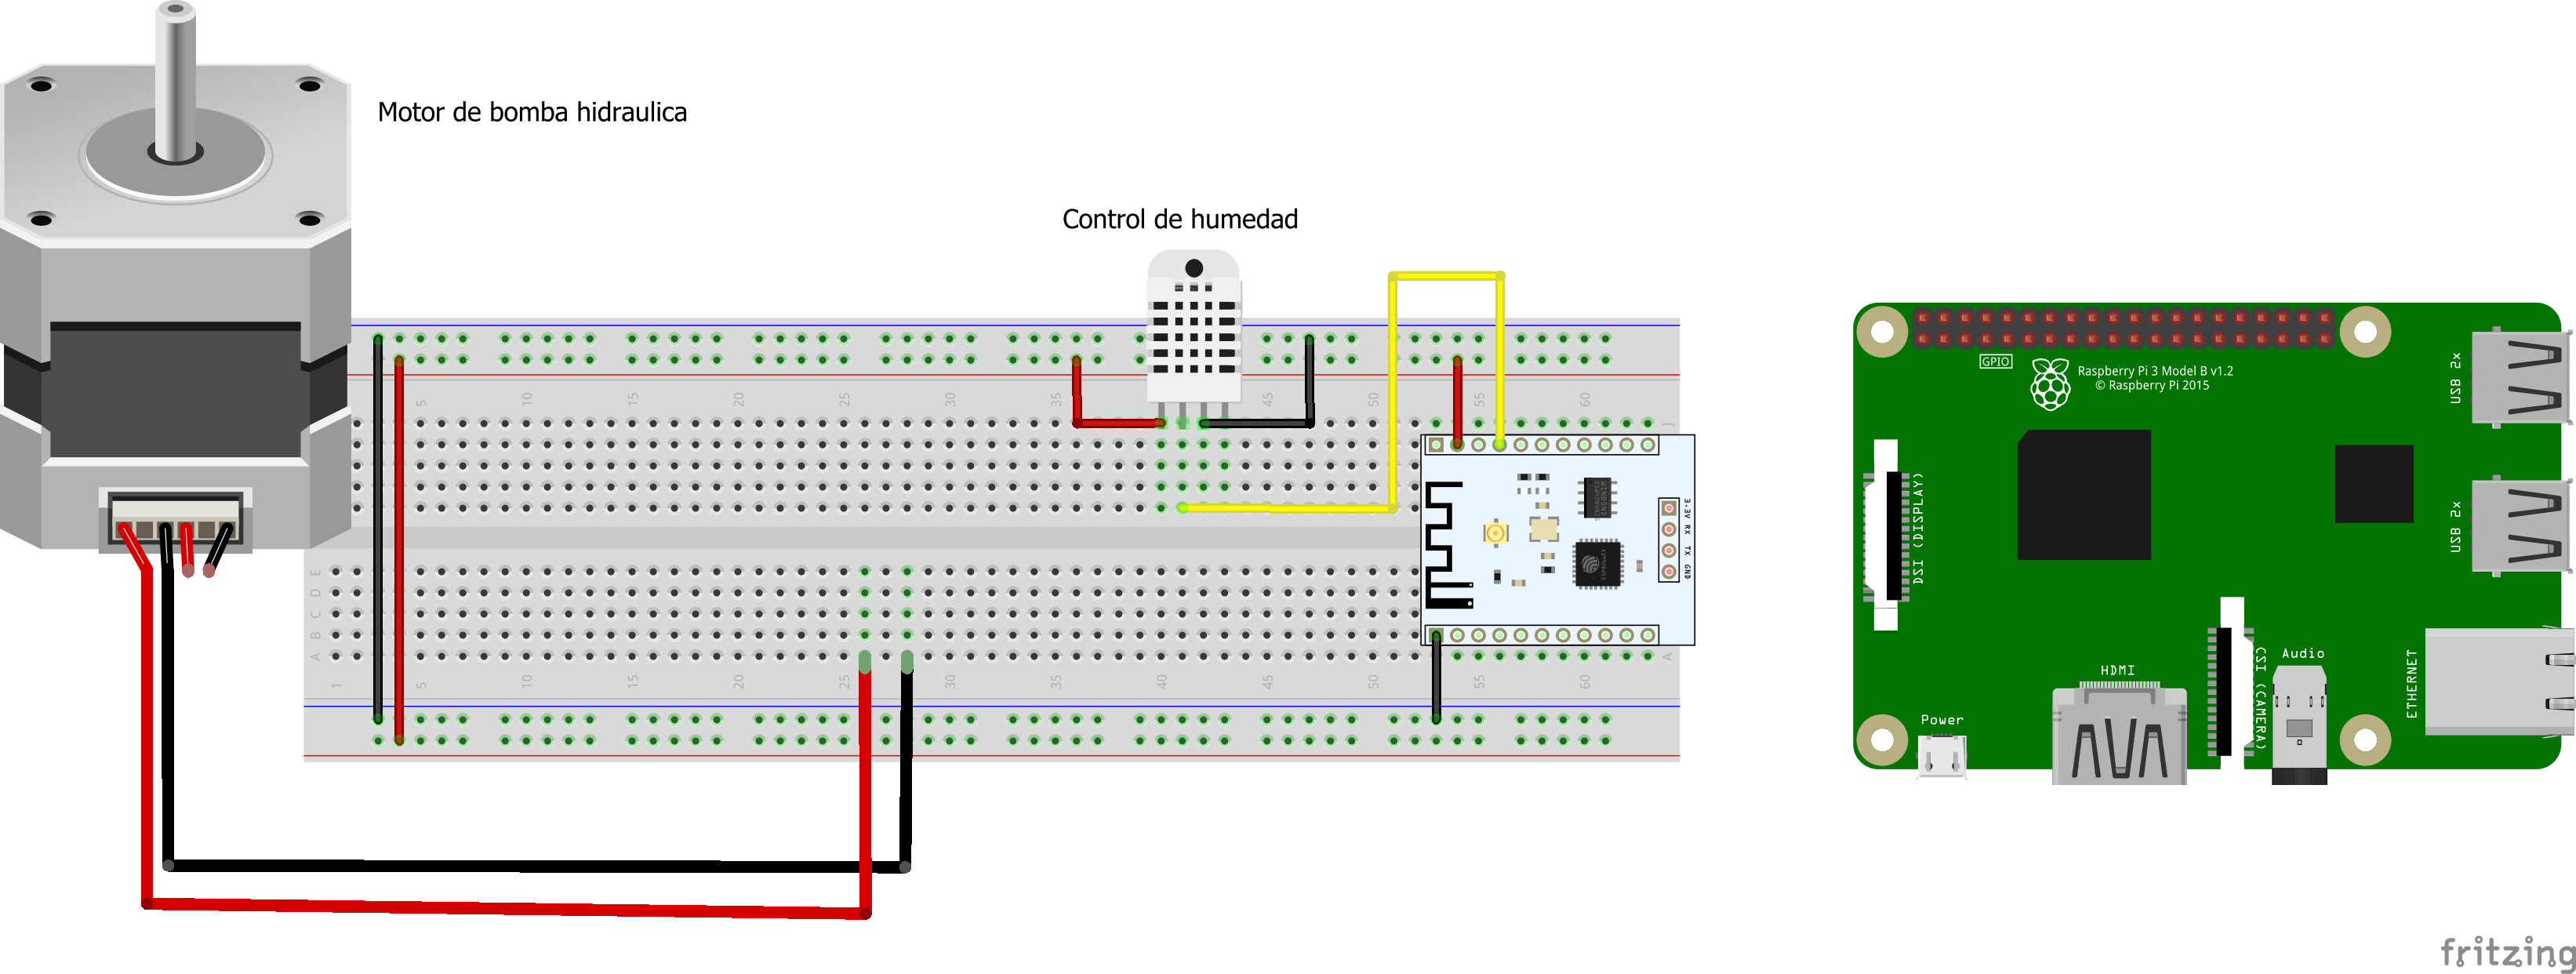
\includegraphics[scale=0.5]{./images/Conexion.png}
		\caption{Esquema básico de conexión Sensor-Sistema-Actuador}
		\label{Esquema_basico}
	\end{figure}		
	
	
	\section{Materiales y Elementos necesarios}
	A continuación se indican los materiales necesarios para la construcción del prototipo, que estará compuesto por una jardinera para los cultivos adaptada al dispositivo IoT desarrollado.\cite{2014}

	\subsection*{Materiales para la construcción de la jardinera}

		\begin{itemize}
			\item Tubos de plástico.
			\item Bandeja donde colocar la planta y verter el agua.
			\item Canalización de plástico donde colocar la planta.
		\end{itemize}			
	
	\subsection*{Sensores}
	Los sensores serán los componentes encargados de medir las condiciones en las que se encuentra el cultivo, en función de varios indicadores.

Alguno de los sensores necesarios, estarán en contacto directo con el agua y por tanto, será necesario que sean sumergibles.\cite{sensores}
		\begin{itemize}
			\item Humedad aire.
			\item Humedad suelo.
			\item Fotovoltaico.
			\item Temperatura.
		\end{itemize}

	\subsection*{Actuadores}

		\begin{itemize}
			\item Bomba de riego.
			\item Interruptor (Encendido y apagado del sistema de forma manual).
		\end{itemize}			
	
	\subsection*{Controladores}
	La lógica del sistema se e ncontrará implementada en los siguientes elementos:
		\begin{itemize}
			\item Raspberry Pi.
			\item ESP8266 | NodemCu.
		\end{itemize}			

	
	\subsection*{Información a tratar}
	En este punto, se describe los flujos de información entre los distintos bloques del sistema.

		\begin{itemize}
			\item \textbf{Sensores-ESP8266:}Los sensores registrarán los datos necesarios para el cultivo, y los enviará al ESP8266.
			\item \textbf{ESP8266-Actuadores:} En función de los valores registrados y al configuración realizada, se enviarán diferentes ordenes desde el ESP8266 a los actuadores para mantener los indicadores en los valores necesarios para el cultivo.
			\item \textbf{ESP8266-RasPi:} El ESP8266 trasladará la información de los indicadores medidos e instrucciones sobre los actuadores a RasPi. La integración entre ambos elementos se efectuará mediante Node-RED.
			\item \textbf{RasPi-ESP8266:} Instrucciones correspondientes a los datos externos recogidos (lluvia, temperatura, iluminación,...) desde Internet. También permite la configuración por parte del usuario y la visualización de los datos recogidos todo ello mediante el uso de Node-RED.
			
		\end{itemize}




\newpage
\section{Presupuesto}

REVISAR

\begin{table}[htbp]
\begin{center}
\begin{tabular}{|l||l|l|}
\hline
Componente & Modelo & Precio (€) \\ \hline \hline
Sensor Humedad &	Glyduino FC-28 &	0,85  \\ \hline
Sensor Fotovoltaico &  GL5549 & 0,15 \\ \hline
Sensor Temperatura & LM35 & 0,85 \\ \hline
Sensor pH & BPSCA K3031LG - HE32389 & 30 \\ \hline
Sensor Conductividad & DIY TDS & 13,15 \\ \hline
ESP8266 & NodeMCU Lua Lolin V3 & 6,49 \\ \hline
Bomba de riego & Mini Bomba de Agua DC 3V -5V Sumergible & 8,79 \\ \hline
Servo Motor (2) & EU-ULN2003 Driver +Step motor & 4,99 \\ \hline
Interruptor & Pulsador switch 12mm & 0,4 \\ \hline
  & TOTAL & 65.67 \\ \hline



\end{tabular}
\caption{Presupuesto Componentes Electrónicos.}
\label{tabla:sencilla}
\end{center}
\end{table}

\chapter{Funcionamiento}

	El funcionamiento del proyecto consistirá en dos partes bien diferenciadas. La primera, está simbolizada en la figura siguiente \ref{Funcionamiento}, donde se irán leyendo los sensores cada cierto tiempo. En caso de necesidad se activarán los actuadores y en caso contrario el dispositivo quedará suspendido hasta que paso el tiempo correspondiente. También se activarán al principio de la ejecución la rutina de interrupción, para permitir qué, en el caso de que el dispositivo esté dormido y el usuario quiera realizar un cambio, se despierte y se realicen los cambios con los actuadores según ordene la placa Raspberry Pi.

	\begin{figure}[H]
		\center
		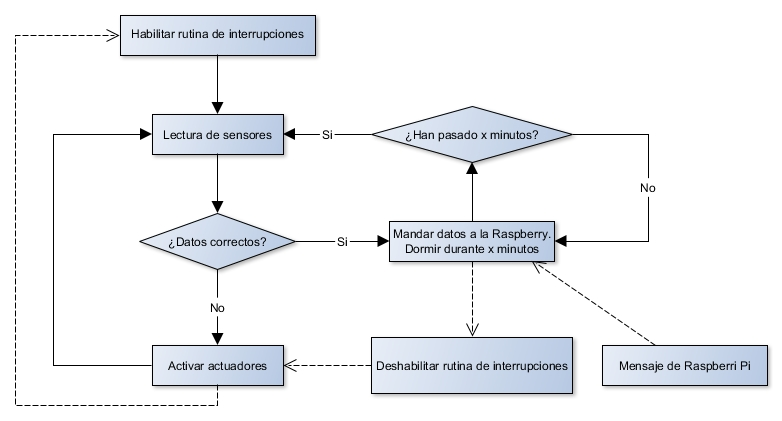
\includegraphics[scale=0.5]{./images/funcionamientoESP8266.jpg}
		\caption{Funcionamiento del módulo ESP8266.}
		\label{Funcionamiento}
	\end{figure}
	
	La placa Raspberry, por el contrario, será la encargada de manejar la Base de Datos (BBDD) donde se almacenarán los datos recogidos por el Esp8266, y la interfaz gráfica con la que el usuario podrá interactuar con el sistema.

\chapter{Listado de tareas para acometer el proyecto }

	En esta sección, se describen las tareas propuestas inicialmente para la ejecución de este proyecto. En cada tarea, a su vez se indicará si se poseen actualmente los conocimientos necesarios o no para afrontar la tarea en concreto.
	
	\subsection*{Elección de los componentes electrónicos adecuados}	
	Consiste en la elección de los modelos concretos de los componentes utilizados principalmente como sensores y actuadores. Antes de adquirir cualquiera de estos dispositivos, se intentarán usar algunos componentes de los que ya disponemos y en el caso de que no sea así, se usar los disponibles en el laboratorio de la asignatura. 

	\subsection*{Programación de los diferentes componentes}
		Programación de la placa Esp8266 con la funcionalidad requerida y, programación y configuración de los diferentes programas de la placa de desarrollo Raspberry Pi.
	
	\subsection*{Cableado del sistema}
	Diseño y preparación del cableado adecuado para la construcción del prototipo. Es posible que se requiera de soldaduras y la necesidad de aislar los componentes electrónicos del agua empleada para el cultivo.

	\subsection*{Construcción del modelo de jardinería}
	Construcción del modelo de jardinería donde se ubicarán los cultivos. Se espera poder construir este modelo con los conocimientos actuales de los miembros del grupo.

	\subsection*{Instalación de los diferentes componentes en la jardinera}
	Integración del modelo de jardinería con el sistema electrónico desarrollado para formar el prototipo final. Es importante tener en cuenta el aislamiento de los componentes electrónicos del agua del modelo de jardinería. No se dispone aún de los conocimientos necesarios.

\subsection*{Definición de una tabla de actuación según valores registrados}
	Definir una tabla de valores umbrales de las medidas obtenidas por los sensores según el tipo de cultivo. Para el tipo de cultivo definido en el prototipo se fijarán los valores óptimos para dicho cultivo y se definirán las acciones a llevar a cabo una vez superados los valores umbrales.
	
	
	\subsection*{Instalación y programación de la API Node-Red}
	Instalar la API Node-Red para la configuración y desarrollo de la interfaz gráfica que será puente entre el usuario y el sistema. Esta GUI, mostrará los datos recogidos de los sensores y tendrá diferentes funcionalidades para que el usuario pueda interactuar con el sistema, cambiado el horario de cambio de agua, encendiendo o apagando el sistema, o cambiado los valores de la planta en caso de que se plante una variedad diferente.
	
	\subsection*{Probar el sistema y solucionar posibles fallos}
	Elaborar plan de pruebas, donde se describan las pruebas a realizar sobre el prototipo desarrollado. A partir de los errores detectados en el plan de pruebas, se deberán de solucionar dichos fallos hasta conseguir una versión final y estable del sistema.
Se dispone de integrantes del grupo con experiencia en elaboración de planes de prueba.
	

\chapter{Ampliaciones}

\subsection*{Alertas y notificaciones al usuario}
	Permitir que el usuario defina una serie de valores umbrales y una vez se sobrepasen dichos valores, este sea avisado vía mail del estado del sistema para que se tomen las medidas necesarias en el caso de que fuesen necesarias.

	\subsection*{Registro de la información en BBDD Mongo DB}
	Diseñar el modelado y programación de la base de datos en el sistema MongoDB, para adaptar este sistema a las necesidades del proyecto. El objetivo es poder almacenar la información recibida en BBDD para en caso de caida del equipo sea posible recuperar los datos registrados o configuración del sistema. La BD Mongo DB se encontrará en instalada con Cloud (https://www.mongodb.com/cloud/atlas).


	\subsection*{Motor de control de persiana o toldo}
	Para controlar la luminosidad del cultivo, se plantea como ampliación la instalación de un motor adicional para el control de la luz natural. Esta ampliación consistirá en la programación y configuración de una persiana móvil, o toldo, con un motor bidireccional. En caso de que haya demasiada luz, la cual pueda llegar a quemar la planta se activará el motor para bajar la persiana o toldo y reducir así la luz que incida en la planta. En caso de que la luz sea insuficiente y sea de día se activará para recoger la persiana o el toldo.
	
	\subsection*{Iluminación artificial}
	Para cultivos de interior o en zonas de poca iluminación, esta ampliación consiste en utilizar un sistema de iluminación artificial controlada por nuestro dispositivo. La ampliación consistiría en garantizar que el cultivo recibe la iluminación necesaria a partir de las lecturas del sensor fotovoltaico, en caso de que no fuera así se encendería el sistema de iluminación.


	\subsection*{Ampliación del tipo de sensores}
	Aunque no está previsto inicialmente, es posible que para determinados cultivos sea necesario usar otro tipo de sensores como por ejemplo un sensor que obtenga la cantidad oxígeno disuelto en agua.




	
\newpage
\addcontentsline{toc}{chapter}{Bibliografía}
\bibliographystyle{plain}
\bibliography{memoria}

\end{document}
